\subsection{XACML}

 \acrfull{xacml} is a standardised, XML-based language for expressing security policies. It provides methods to define and combine security policies and to rapidly identify, which policy applies to a given subject. \acrshort{xacml} was first standardised by OASIS\footnote{\url{https://www.oasis-open.org/}, accessed 04 March 2019} in 2003 and the latest version is XACML 3.0, standardised in 2013~\cite{OASISStandard2013EXtensible3.0}. The further description is based on this latest version.
 
 The context of \acrshort{xacml} is illustrated in Figure~\ref{fig:xacml-context}. At the centre of the system is the \acrfull{pdp} which evaluates an input (such as access requests) against a policy set and issues an output -- a decision (such as \textit{access granted}). \acrshort{xacml} defines the formal language of the policy set and of the requests/responses. A policy set contains comprises one or more \textit{policies} and a \textit{policy combining algorithm}. The main components of a policy are a \textit{target} to which this policy applies and one or more \textit{rules}. The rule must specify a \textit{target} to which it applies and an \textit{evaluation} (\textit{permit} or \textit{deny}). It can also optionally specify \textit{conditions}, \textit{obligations} and \textit{advices}, all of which further shape the scope of the rule. Policy combining algorithm specifies the order and other conditions that decide, which policy will be finally applied on the request~\cite{OASISStandard2013EXtensible3.0}.
 
 \begin{figure}[ht]
    \centering
    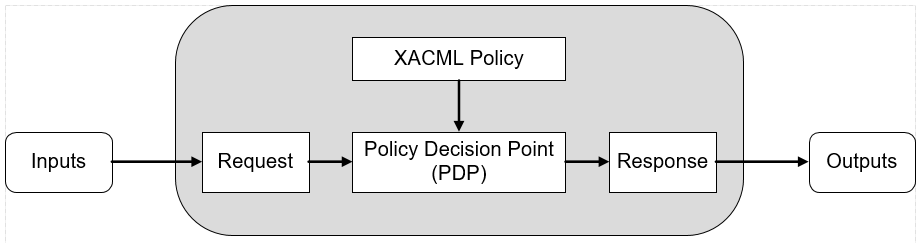
\includegraphics[width=.95\textwidth]{xacml-context}
    \caption{The context diagram of \acrshort{xacml}. From~\cite{OASISStandard2013EXtensible3.0}, edited.
    }
    \label{fig:xacml-context}
\end{figure}
 
The \acrshort{xacml} standard defines in detail several logical entities and their interactions. The native format for messages between these entities is XML, but a profile has been developed to support JSON message format~\cite{2017JSON1.0}. Additional profile was also created to describe implementation in a RESTful architecture~\cite{2017REST1.0}.
 
 Several implementations of \acrshort{xacml} exist in Java, Python and other languages. Criticisms of \acrshort{xacml} include low adoption rate, unsuitability for federated enterprises~\cite{Cser2013XACMLDead}, and lack of transparency for the end user~\cite{Cser2013XACMLDead, Ardagna2011ExpressiveApplications}.

